\documentclass{article}
\usepackage[final]{nips_2017}
\usepackage[utf8]{inputenc} % allow utf-8 input
\usepackage[T1]{fontenc}    % use 8-bit T1 fonts
\usepackage{csquotes}
\usepackage{hyperref}       % hyperlinks
\usepackage{url}            % simple URL typesetting
\usepackage{booktabs}       % professional-quality tables
\usepackage{amsfonts}       % blackboard math symbols
\usepackage{nicefrac}       % compact symbols for 1/2, etc.
\usepackage{microtype}      % microtypography
\usepackage{graphicx}
\usepackage{longtable}
\usepackage{xspace}
\usepackage[section]{placeins}
%\usepackage[rm={lining,proportional},sf={lining,proportional},tt={lining,proportional,variable}]{cfr-lm}
%\usepackage{cfr-lm} % old-figure aribic numerals1\

\usepackage{tikz}
\usetikzlibrary{tikzmark}
\usetikzlibrary{arrows,arrows.meta,decorations.pathreplacing,shapes}
\newcommand{\Concat}[2]{\ensuremath{\texttt{#1}\,\mathbin\Vert\,\texttt{#2}}}
\tikzstyle{arrow} = [draw, very thick, color=black!50, -{Latex[scale=0.75]}]


\bibliographystyle{abbrvnat}

%\makesavenoteenv{longtable}
\UseMicrotypeSet[protrusion]{basicmath}
\providecommand{\tightlist}{%
	\setlength{\itemsep}{0pt}\setlength{\parskip}{0pt}}
\setcounter{secnumdepth}{-\maxdimen}

\newcommand{\Num}[1]{\oldstylenums{#1}}
\newcommand{\CR}{\ensuremath{\mathbf{CR}}\xspace}
\newcommand{\TER}{\ensuremath{\mathbf{TER}}\xspace}
\newcommand{\TERC}{\ensuremath{\mathbf{TERC}}\xspace}
\newcommand{\DnD}{D\&D 5e\xspace}
\newcommand{\TierLeast}{\ensuremath{\textsc{Least}}\xspace}
\newcommand{\TierLess}{\ensuremath{\textsc{Less}}\xspace}
\newcommand{\TierFair}{\ensuremath{\textsc{Fair}}\xspace}
\newcommand{\TierMore}{\ensuremath{\textsc{More}}\xspace}
\newcommand{\TierMost}{\ensuremath{\textsc{Most}}\xspace}
\newcommand{\FiveETools}{\href{https://5etools-mirror-1.github.io/}{\texttt{5e.tools}}\xspace}
\newcommand{\DnDCombat}{\texttt{dndcombat.com}\xspace}
\newcommand{\Column}[1]{\ensuremath{\texttt{\textquotesingle{}#1\textquotesingle{}}}\xspace}
\newcommand{\IndexRange}[2]{\ensuremath{\texttt{{[}\,#1,\ #2\,{]}}}\xspace}
\newcommand{\NumericRange}[2]{\ensuremath{\left[\,#1,\; #2\,\right]}\xspace}
\newcommand{\TierTrivial}{\ensuremath{\textsc{``Trivial''}}\xspace}
\newcommand{\TierCosmic}{\ensuremath{\textsc{``Cosmic''}}\xspace}

\title{Comparative Combat Categories in\\Dungeons and Dragons 5th Edition\\[5mm]\normalsize CSc 74020 Project Proposal --- \today}

\author{
  Alex Washburn\thanks{\url{https://recursion.ninja}} \\
  Department of Computer Science\\
  CUNY Graduate Center\\
  \texttt{awashburn@gc.cuny.edu} \\
  \And
  Gibeom Park\\
  Department of Computer Science\\
  CUNY Graduate Center\\
  \texttt{gpark1@gc.cuny.edu} \\
  %% Coauthor \\
  %% examples of more authors
  %% Affiliation \\
  %% Address \\
  %% \texttt{email} \\
  %% \AND
  %% Coauthor \\
  %% Affiliation \\
  %% Address \\
  %% \texttt{email} \\
  %% \And
  %% Coauthor \\
  %% Affiliation \\
  %% Address \\
  %% \texttt{email} \\
  %% \And
  %% Coauthor \\
  %% Affiliation \\
  %% Address \\
  %% \texttt{email} \\
}

\begin{document}
% \nipsfinalcopy is no longer used

%\begin{center}
%\includegraphics[width=3cm, height=0.7cm]{CS230}
%\end{center}

\maketitle

\begin{abstract}
The project explores the applicability of machine learning classifiers as a proposed substitute for the deficient monster Challenge Rating defined in Dungeons and Dragons 5th Edition.
Multiple supervised learning models will be trained on a dataset of monster features listed Dungeons and Dragons.
Monster Elo scores will be used as labels.
The project's resulting classifiers will predict a monster's lethality, ordering them into five tiers.
\end{abstract}

\section{Introduction}


\subsection{Challenge Rating}

We propose that we explore an under-developed aspect of Dungeons and Dragons 5th Edition (\DnD), the monster "Challenge Rating" system.
The Challenge Rating (\CR) is a measure of an individual monster’s lethality to a party of four characters.
The challenge rating system is described in the \DnD \emph{Monster Manual} \cite{DnD5eMonsterManual2014} in the following excerpt:

\begin{displayquote}
	A monster's \textbf{challenge rating} tells you how great a threat the monster is.
	An appropriately equipped and well-rested party of four adventurers should be able to
	defeat a monster that has a challenge rating equal to its level without suffering any deaths.
	For example, a party of four 3rd-level characters should find a monster with a challenge rating of 3 to be a worthy challenge, but not a deadly one.
\end{displayquote}

In a supplementary \DnD work, \emph{Xanathar's Guide to Everything} \cite{DnD5eXanathars2017}, the \CR system is elaborated on further:

\begin{displayquote}
	The above guidelines are designed to create a fight that will challenge a party while still being winnable.
	If you want to create an easier encounter that will challenge characters but not threaten to defeat them, you can treat the party as if it were roughly one-third smaller than it is.
	For example, to make an easy encounter for a party of five characters, put them up against monsters that would be a tough fight for three characters.
	Likewise, you can treat the party as up to half again larger to build a battle that is potentially deadly, though still not likely to be an automatic defeat.
	A party of four characters facing an encounter designed for six characters would fall into this category.
\end{displayquote}

It is clear from the source material descriptions that if a baseline part of four characters is used, then when party level is same level as the monster's \CR the encounter lethality is considered ``worthy,'' where as a monster with \CR \emph{two less} than the party level being considered``easy'' and \CR \emph{two greater} is ``deadly.''
Unfortunately, the official \CR values that have been published are more often than not poor estimates of monster lethality in practice.


\subsection{Proposed Solution}

%In this project, we propose producing an substitute ranking of monster lethality, ordering them into \emph{five tiers} $\left[\;\TierLeast,\,\TierLess,\,\TierFair,\,\TierMore,\,\TierMost\;\right]$.
In this project, we propose producing an substitute ranking of monster lethality.
The original \CR ranking system is ``semi-logarithmic,''and reminiscent of the Elo ranking system \cite{elo1978rating}.
Unsurprisingly, the calculation of \DnD Elo ranks has been preformed by other.
Hence it seems natural that the substituted lethality system ought to be based on the more flexible Elo ranking system.
We propose two options involving machine learning predictors for \DnD monster lethality.
The predictor will process a \DnD monster's features and predict the monster's lethality based on the Elo ranking.


\subsubsection{Option 1: Greater effort, greatest precision}

One solution would be for a players to ignore the concept of the \CR system from the core material entirely 
Instead, when playing \DnD a specific party's Elo rank can be tracked based on their successful and unsuccessful encounters.
Future encounters can be designed to a desired level of lethality by considering the part's current Elo Rank and selecting monsters with appropriately similar Elo ranks.
The authors conjecture that in practice, the adoption of Elo rank tracking in conjunction with the application of machine learning will produce a better indicator of monster lethality than the conceptual framework of the \CR system.

However, this solution requires the players to be familiar with Elo's algorithm, as well as having access to Elo ranks of all possible \DnD monsters.
Furthermore, it requires a willingness for the players to learn and maintain adjusted Elo ranking for the party and \DnD monsters.
While this solution provides the most precision when estimating lethality for a particular party, the ``barrier to access'' is likely too great for the typical players.
Due to this, we do not explore this solution and instead propose a more accessible solution instead.


\subsubsection{Option 2: Minimal effort, still great precision}

Our proposed solution is the creation of an alternative tiered ranking system philosophically analogous to the \CR system, but based on empirical derived Elo ranks rather than the published \CR ranks estimated by human authors.
The classes of the official \CR system are depicted in Figure \ref{fig:CR-Classes}.
For our replacement system, we desire an \Column{Elo Tier} column to be represented as an discrete ordinal class.
The creation of a companion machine learning classifier to place novel \DnD monsters into the most appropriate class will minimize the ``barrier to access'' while still conferring the precision of empirical Elo rank computations to players.

In this work we construct two substitution candidates for the \CR system analyze the predictive efficacy of classifiers trained via supervised learning.
The first candidate system is the Tiered Elo Rank (\TER), with\Num{22} classes.
The second candidate system is the Tiered Elo Rank (Compressed) (\TERC), with \Num{12} classes.
Both candidates have a corresponding morphism to the \CR system illustrated in Figure \ref{fig:CR-Mapping}.
In both candidates the morphism collapses the ``trivial'' and ``epic'' ranges of the \CR system into single classes.
There is a one-to-one correspondence of the ``character level'' classes of the \CR system to a classes in the \TER candidate system.
However, there is a \emph{two}-to-one correspondence of the ``character level'' classes of the \CR system to a classes in the \TERC candidate system.
This makes \TERC a more granular candidate but potentially more difficult to predict, where as \TERC is less granular but potentially easier to predict.
In our project we evaluate the predictive power of multiple machine learning algorithms when given tasked with classifying an novel \DnD monster to it's corresponding \TER and \TERC class.


\begin{figure}[htb]
\centering
\resizebox{\textwidth}{!}{%\documentclass[tikz]{standalone}
%\usepackage{tikz}
%\usetikzlibrary{decorations.pathreplacing,shapes}

%\begin{document}
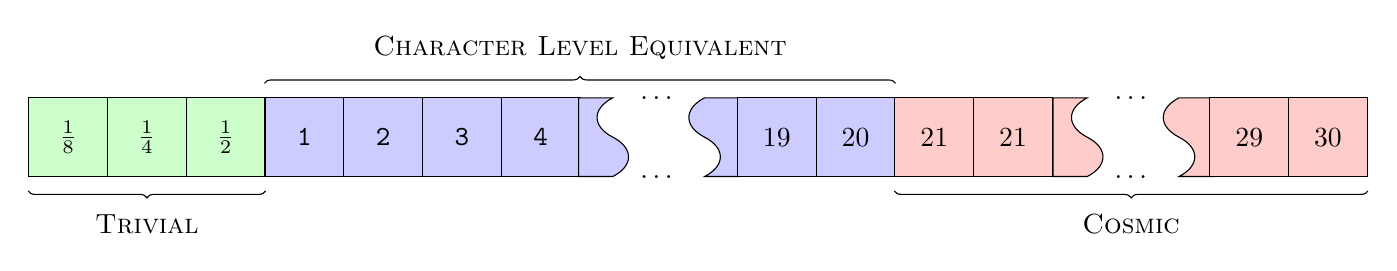
\begin{tikzpicture}[auto]
\foreach \c/\i [count=\n] in  
{green!20/$\frac{1}{8}$,green!20/$\frac{1}{4}$,green!20/$\frac{1}{2}$,blue!20/1,blue!20/2,blue!20/3,blue!20/4}
\node[draw,fill=\c,minimum height=1cm,minimum width = 1cm,xshift=\n*1cm,font=\ttfamily](NP\n){\i} ;

\draw [decoration={brace,mirror,raise=5pt},decorate] (NP1.south west) -- node[below=10pt]{$\textsc{Trivial}$}(NP3.south east);

\node [tape, draw,,fill=blue!20,minimum height=0.5cm,minimum width = 1cm,tape bend top=none,
tape bend height=0.4cm,rotate=90] at (7.6,0) (t) {};
\node [tape, draw,,fill=blue!20,minimum height=0.5cm,minimum width = 1cm,tape bend top=none,
tape bend height=0.4cm,rotate=270] at (9.4,0) (t) {};

\node at (8.5, 0.5) {\dots};
\node at (8.5,-0.5) {\dots};

\foreach \c/\i [count=\m] in  
{blue!20/19,blue!20/20,red!20/21,red!20/21} 
\node[draw,fill=\c,minimum height=1cm,minimum width = 1cm,xshift=9cm+\m*1cm](NS\m){\i} ;
%\draw [decoration={brace,mirror,raise=5pt},decorate] (N2.south west) --  node[below=10pt]{$M_d$}(N2.south east); 

\node [tape, draw,,fill=red!20,minimum height=0.5cm,minimum width = 1cm,tape bend top=none,
tape bend height=0.4cm,rotate=90] at (13.625,0) (t) {};
\node [tape, draw,,fill=red!20,minimum height=0.5cm,minimum width = 1cm,tape bend top=none,
tape bend height=0.4cm,rotate=270] at (15.425,0) (t) {};

\node at (14.525, 0.5) {\dots};
\node at (14.525,-0.5) {\dots};

\foreach \c/\i [count=\m] in  
{red!20/29,red!20/30} 
\node[draw,fill=\c,minimum height=1cm,minimum width = 1cm,xshift=15cm+\m*1cm](NT\m){\i} ;
\draw [decoration={brace,raise=5pt},decorate] (NP4.north west) --  node[above=10pt]{$\textsc{Character Level Equivalent}$} (NS2.north east); 

\draw [decoration={brace,mirror,raise=5pt},decorate] (NS3.south west) -- node[below=10pt]{$\textsc{Cosmic}$}(NT2.south east);

\end{tikzpicture}

%\end{document}
}
\caption{Official \CR classes for \DnD monsters.}\label{fig:CR-Classes}
\end{figure}


\begin{figure}[htb]
\centering
\resizebox{\textwidth}{!}{%\documentclass[tikz]{standalone}
%\usepackage{tikz}
%\usetikzlibrary{tikzmark}
%\usetikzlibrary{arrows,arrows.meta,decorations.pathreplacing,shapes}

%\newcommand{\Concat}[2]{\ensuremath{\texttt{#1}\,\mathbin\Vert\,\texttt{#2}}}

%\tikzstyle{arrow} = [draw, very thick, color=black!50, -{Latex[scale=0.75]}]


%\begin{document}
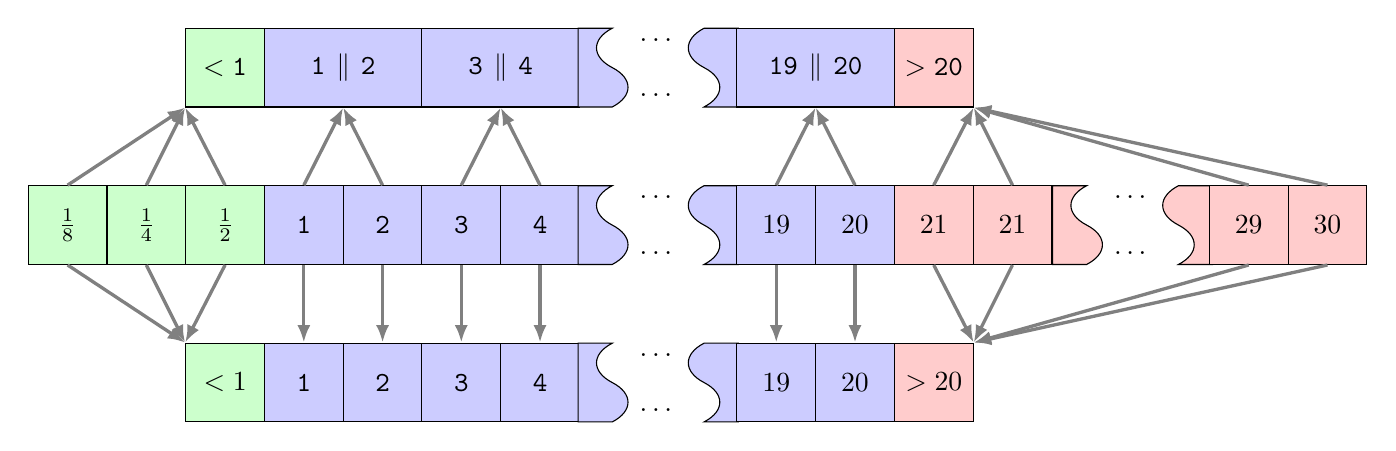
\begin{tikzpicture}[auto]


%%% %%%
% TERC
%%% %%%


\node[draw,fill=green!20,minimum height=1cm,minimum width = 1cm,yshift=2cm,xshift=3cm,font=\ttfamily](TERCNP0){$< \texttt{1}$};

\foreach \c/\i [count=\n] in 
{blue!20/\Concat{1}{2},blue!20/\Concat{3}{4}}
\node[draw,fill=\c,minimum height=1cm,minimum width = 2cm,yshift=2cm,xshift=\n*2cm + 2.5 cm,font=\ttfamily](TERCNP\n){\i} ;

\node [tape, draw,,fill=blue!20,minimum height=0.5cm,minimum width = 1cm,yshift=2cm,tape bend top=none, tape bend height=0.4cm,rotate=90] at (7.6,0) (t) {};
\node [tape, draw,,fill=blue!20,minimum height=0.5cm,minimum width = 1cm,yshift=2cm,tape bend top=none, tape bend height=0.4cm,rotate=270] at (9.4,0) (t) {};

\node[yshift=2cm] at (8.5, 0.35) {\dots};
\node[yshift=2cm] at (8.5,-0.35) {\dots};

\node[draw,fill=blue!20,minimum height=1cm,minimum width = 2cm,yshift=2cm,xshift=10.5cm,font=\ttfamily](TERCNS1){\Concat{19}{20}};

\node[draw,fill=red!20,minimum height=1cm,minimum width = 1cm,yshift=2cm,xshift=12cm,font=\ttfamily](TERCNS2){$> \texttt{20}$};

%\foreach \c/\i [count=\m] in  
%{blue!20/19,blue!20/20,red!20/$> 20$} 
%\node[draw,fill=\c,minimum height=1cm,minimum width = 1cm,yshift=2cm,xshift=9cm+\m*1cm](NS\m){\i} ;


%%% %%%
% CR 
%%% %%%


\foreach \c/\i [count=\n] in  
{green!20/$\frac{1}{8}$,green!20/$\frac{1}{4}$,green!20/$\frac{1}{2}$,blue!20/1,blue!20/2,blue!20/3,blue!20/4}
\node[draw,fill=\c,minimum height=1cm,minimum width = 1cm,xshift=\n*1cm,font=\ttfamily](CRNP\n){\i} ;

\node [tape, draw,,fill=blue!20,minimum height=0.5cm,minimum width = 1cm,tape bend top=none, tape bend height=0.4cm,rotate=90] at (7.6,0) (t) {};
\node [tape, draw,,fill=blue!20,minimum height=0.5cm,minimum width = 1cm,tape bend top=none, tape bend height=0.4cm,rotate=270] at (9.4,0) (t) {};

\node at (8.5, 0.35) {\dots};
\node at (8.5,-0.35) {\dots};

\foreach \c/\i [count=\m] in  
{blue!20/19,blue!20/20,red!20/21,red!20/21} 
\node[draw,fill=\c,minimum height=1cm,minimum width = 1cm,xshift=9cm+\m*1cm](CRNS\m){\i} ;

\node [tape, draw,,fill=red!20,minimum height=0.5cm,minimum width = 1cm,tape bend top=none, tape bend height=0.4cm,rotate=90] at (13.625,0) (t) {};
\node [tape, draw,,fill=red!20,minimum height=0.5cm,minimum width = 1cm,tape bend top=none, tape bend height=0.4cm,rotate=270] at (15.425,0) (t) {};

\node at (14.525, 0.35) {\dots};
\node at (14.525,-0.35) {\dots};

\foreach \c/\i [count=\m] in  
{red!20/29,red!20/30} 
\node[draw,fill=\c,minimum height=1cm,minimum width = 1cm,xshift=15cm+\m*1cm](CRNT\m){\i} ;


%%% %%%
% TER
%%% %%%


\foreach \c/\i [count=\n] in  
{green!20/$< 1$,blue!20/1,blue!20/2,blue!20/3,blue!20/4}
\node[draw,fill=\c,minimum height=1cm,minimum width = 1cm,yshift=-2cm,xshift=(\n+2)*1cm,font=\ttfamily](TERNP\n){\i} ;

\node [tape, draw,,fill=blue!20,minimum height=0.5cm,minimum width = 1cm,yshift=-2cm,tape bend top=none, tape bend height=0.4cm,rotate=90] at (7.6,0) (t) {};
\node [tape, draw,,fill=blue!20,minimum height=0.5cm,minimum width = 1cm,yshift=-2cm,tape bend top=none, tape bend height=0.4cm,rotate=270] at (9.4,0) (t) {};

\node[yshift=-2cm] at (8.5, 0.35) {\dots};
\node[yshift=-2cm] at (8.5,-0.35) {\dots};

\foreach \c/\i [count=\m] in  
{blue!20/19,blue!20/20,red!20/$> 20$} 
\node[draw,fill=\c,minimum height=1cm,minimum width = 1cm,yshift=-2cm,xshift=9cm+\m*1cm](TERNS\m){\i} ;


%%%
% Arrows: Trivial
%%%


\draw [arrow] (CRNP1.north) to (TERCNP0.south west);
\draw [arrow] (CRNP2.north) to (TERCNP0.south west);
\draw [arrow] (CRNP3.north) to (TERCNP0.south west);

\draw [arrow] (CRNP1.south) to (TERNP1.north west);
\draw [arrow] (CRNP2.south) to (TERNP1.north west);
\draw [arrow] (CRNP3.south) to (TERNP1.north west);


%%%
% Arrows: Cosmic
%%%

\draw [arrow] (CRNS3.north) to (TERCNS2.south east);
\draw [arrow] (CRNS4.north) to (TERCNS2.south east);
\draw [arrow] (CRNT1.north) to (TERCNS2.south east);
\draw [arrow] (CRNT2.north) to (TERCNS2.south east);

\draw [arrow] (CRNS3.south) to (TERNS3.north east);
\draw [arrow] (CRNS4.south) to (TERNS3.north east);
\draw [arrow] (CRNT1.south) to (TERNS3.north east);
\draw [arrow] (CRNT2.south) to (TERNS3.north east);


%%%
% Arrows: Equivelent Range
%%%

\draw [arrow] (CRNP4.north) to (TERCNP1.south);
\draw [arrow] (CRNP5.north) to (TERCNP1.south);
\draw [arrow] (CRNP6.north) to (TERCNP2.south);
\draw [arrow] (CRNP7.north) to (TERCNP2.south);
\draw [arrow] (CRNS1.north) to (TERCNS1.south);
\draw [arrow] (CRNS2.north) to (TERCNS1.south);

\draw [arrow] (CRNP4.south) to (TERNP2.north);
\draw [arrow] (CRNP5.south) to (TERNP3.north);
\draw [arrow] (CRNP6.south) to (TERNP4.north);
\draw [arrow] (CRNP7.south) to (TERNP5.north);
\draw [arrow] (CRNS1.south) to (TERNS1.north);
\draw [arrow] (CRNS2.south) to (TERNS2.north);


\end{tikzpicture}
%\end{document}
}
\caption{Mapping from \CR classes to \TER(below) and \TERC (above) classes.}\label{fig:CR-Mapping}
\end{figure}


\section{Related work}
Some work has been done on applying ML to table top role playing games (TTRPGs) in the past \cite{rameshkumar2020storytelling, macinnes2019d, cavanaugh2016machine, faria2019adaptive, riedl2013interactive}.
Much of the work revolves around the more tractable problem of selecting appropriate ambient music choices for players to experience based on the current emotional tone of the game \cite{ferreira2017mtg, risi2020increasing, padovani2017bardo, ferreira2020computer}.
However, the most popular TTRPG, Dungeons and Dragons (\DnD) has been used as a difficult test-bed for ML experimentation \cite{martin2018dungeons}.
This particular previous work, while quite notable, focused entirely on non-combat aspects of \DnD, eschewing a core component and past time of \DnD; resolving conflict via numerical simulation.
In our project we will grapple with this numeric aspect of \DnD, focusing on a small subset of the \DnD combat system; quantifying the relative lethality of a monster.
To the best of the author's knowledge, the proposed project will be the first serious attempt to apply machine learning to a numerical aspect of \DnD.
Consequently, there is no \emph{known} previous on which to draw a comparison.


\section{Dataset and Features}

\hypertarget{the-dd-monster-data}{%
	\subsection{D\&D Monster Data}\label{the-dd-monster-data}}

Given the close resemblance between the philosophies of the \CR and the Elo ranking systems, it is not surprising that others have considered applying Elo's ranking algorithm to \DnD monsters.
In fact, these exists a pre--computed Elo score for most \DnD monsters compiled online and continually updated by \DnDCombat \cite{DnDCombat}.
These Elo ranks will serve as labels for supervised learning.
Additionally, a large data-set of \DnD monsters has been pre--compiled online by \FiveETools \cite{Mirror5eTools}
We assemble a rich \DnD monster data-set by linking the measurements from \FiveETools with Elo-ranking labels from \DnDCombat via string matching on monster name .


\hypertarget{datset-assembly}{%
\subsection{Dataset Assembly}\label{datset-assembly}}

The \FiveETools database contains the stat-block records for \Num{2333} \DnD monsters.
Each stat-block is interpreted as a robust feature set of \Num{71} measurements.
Notably, the \FiveETools database contains \emph{zero} missing values for \emph{all} \Num{2333} \DnD monsters.

The \DnDCombat website contained Elo rankings for \Num{2936} \DnD monsters.
Only pairings of monster name and Elo rank were considered from \DnDCombat.
The Elo observations were taken on \texttt{2022-10-25}.


Both the data from \FiveETools and \DnDCombat were retrieved in \href{https://en.wikipedia.org/wiki/JSON}{JSON format}.
The data was parsed and curated using a custom tool written by the authors.
The tool is named \texttt{curate-json} and is written in \href{https://www.haskell.org/}{Haskell}.
In order to build the \texttt{curate-json} tool, the \href{https://www.haskell.org/}{Haskell} compiler \href{https://www.haskell.org/ghc/download.html}{GHC} and build tool \href{https://www.haskell.org/cabal/download.html}{\texttt{cabal}}
are required. 

Exact string matching was used to link the feature records of \FiveETools with the recorded Elo ranking labels of \DnDCombat.
The matching resulted in \Num{1630} linked records.
The size of the matched dataset was deemed sufficient by the authors for the purposes of the study.
Consequently, more flexible matching approaches, such as fuzzing matching, were not attempted.
Matching information is summarized in Table \ref{tab:matching}.


Finally, a search for duplicate records is performed
A total of \Num{248} \DnD monsters with identical name and Elo rankings were discovered.
Inspection of the duplicate records revealed only slight differences between the observations, typically only differing in one of the binary indicator fields.
The observation with the most information, meaning the record with the most binary indicators set, was preserved and the less informative duplicates were dropped.
The deduplicated dataset consists of \Num{1382} observations.

\begin{quote}
\emph{Note that important digital objects exist within the project repository for reference:}%
\end{quote}

\begin{enumerate}

\item 
The source code for the \texttt{curate-json} tool:

\begin{itemize}
	\tightlist
	\item
	\href{https://github.com/recursion-ninja/CSc-74020/tree/master/src/curation}{\texttt{src/curation/*}}
\end{itemize}

\item
The raw data:

\begin{itemize}
	\tightlist
	\item
	\href{https://github.com/recursion-ninja/CSc-74020/tree/master/data/5e.tools}{\texttt{data/5e.tools/*}
	}
	\item
	\href{https://github.com/recursion-ninja/CSc-74020/tree/master/data/dndcombat.com}{\texttt{data/dndcombat.com/*}}
\end{itemize}

\item
The assembled dataset:

\begin{itemize}
	\tightlist
	\item
	\href{https://github.com/recursion-ninja/CSc-74020/tree/master/data/dnd-5e-monsters.csv}{\texttt{data/dnd-5e-monsters.csv}}
\end{itemize}

\end{enumerate}


\hypertarget{input-summary}{
\subsection{Input Summary}\label{input-summary}}

The curated
\href{https://github.com/recursion-ninja/CSc-74020/tree/master/data/dnd-5e-monsters.csv}{\texttt{data/dnd-5e-monsters.csv}} dataset has \Num{1382} rows and \Num{72} columns, constituting the project's initial observations and measurements, respectively.

There are two leading textual columns, labeled \Column{Name} and \Column{Type} indexed
\IndexRange{0}{1}.
The subsequent \texttt{20} columns indexed \IndexRange{2}{21} are "continuous," integral-valued measurements of common \DnD attributes.
The final \Column{Elo\ Rank} column indexed \texttt{71} is the basis for the subsequently extracted supervised learning label.
The next three columns from the end are labeled \Column{Damage\ Tags}, \Column{Spellcasting\ Tags} and \Column{Trait\ Tags} indexed \IndexRange{66}{70}.
The remaining columns indexed \IndexRange{22}{67} are binary indicators for various \DnD monster attributes.
A column summary of the initial data set is presented in Table \ref{tab:initial-dataset}.

\hypertarget{feature-extraction}{%
\subsection{Feature Extraction}\label{feature-extraction}}

\begin{quote}
	{\itshape With a basic understanding of the dataset, we begin feature extraction.}
\end{quote}


\hypertarget{extraction-of-tiers}{
\subsubsection{Tiers Class Labeling}\label{extraction-of-tiers}}

The most important feature extraction involves discretizing the \Column{Elo Rank} values into an ordinal \Column{Tier} class column.
The number of ordinal classes will range from \NumericRange{0}{11} for the \TERC candidate system and \NumericRange{0}{21} for the \TER candidate.
We extract the ordinal values via a two-step procedure.


\subsubsection{Outlier isolation}

First, a threshold $\mathcal{T}$ is identified separating outliers on the upper end of the range from the normally distributed values within \Column{Elo Rank} column.
The \DnD monsters with Elo rankings $r \ge \mathcal{T}$ are extremely powerful, and their granular classification is generally not useful for players.
Rather, inclusion of these \DnD monsters in an encounter is a matter of appropriateness as a story-concluding encounter rather than consideration in designing an interluding encounter.
Therefore we manually classify all \DnD monsters with an Elo ranking $r \ge \mathcal{T}$ as \TierCosmic tier.
The \TierCosmic is encoded as $11$ for \TERC and $21$ for \TER.


\subsubsection{Classes partitioned by clustering}

Secondly, the remaining normally distributed \DnD monsters with Elo ranking $r < \mathcal{T}$ are partitioned into $n - 1$ tiers, either \Num{11} ranging from \NumericRange{0}{10} for \TERC or \Num{21} ranging from \NumericRange{0}{20} for \TER.
The partitions of the normally distributed data conjoined with the manually partitioned outliers of the \TierCosmic results in the desired ordinal classes ranging from \NumericRange{0}{11} for the \TERC and \NumericRange{0}{21} for \TER.
Partitioning of the normally distributed \DnD monsters is performed by K-means clustering into $n - 1$ bins.
The resulting clusters are encoded as ordinal values in ascending order of the bin's mean value.


\subsubsection{Input value and output class distributions}

The distribution of Elo ranking values in dataset is roughly normal, when omitting outliers.
After extracting tier classes via outlier isolation and k-means clustering, the output tier classes account for roughly the same size range of input Elo rank values.
The exceptions which prove the rule are the classes with ordinal values $0$, $n- 2$, and $n - 1$.
However this is not surprising as these classes contain outlier measurements.
The Elo rank distribution and resulting partitions for \TERC and \TER are delineated in Figures \ref{fig:Partitions-TERC} \ref{fig:Partitions-TER}, respectively.
 
\begin{figure}[htb]
	\centering
	\resizebox{\textwidth}{!}{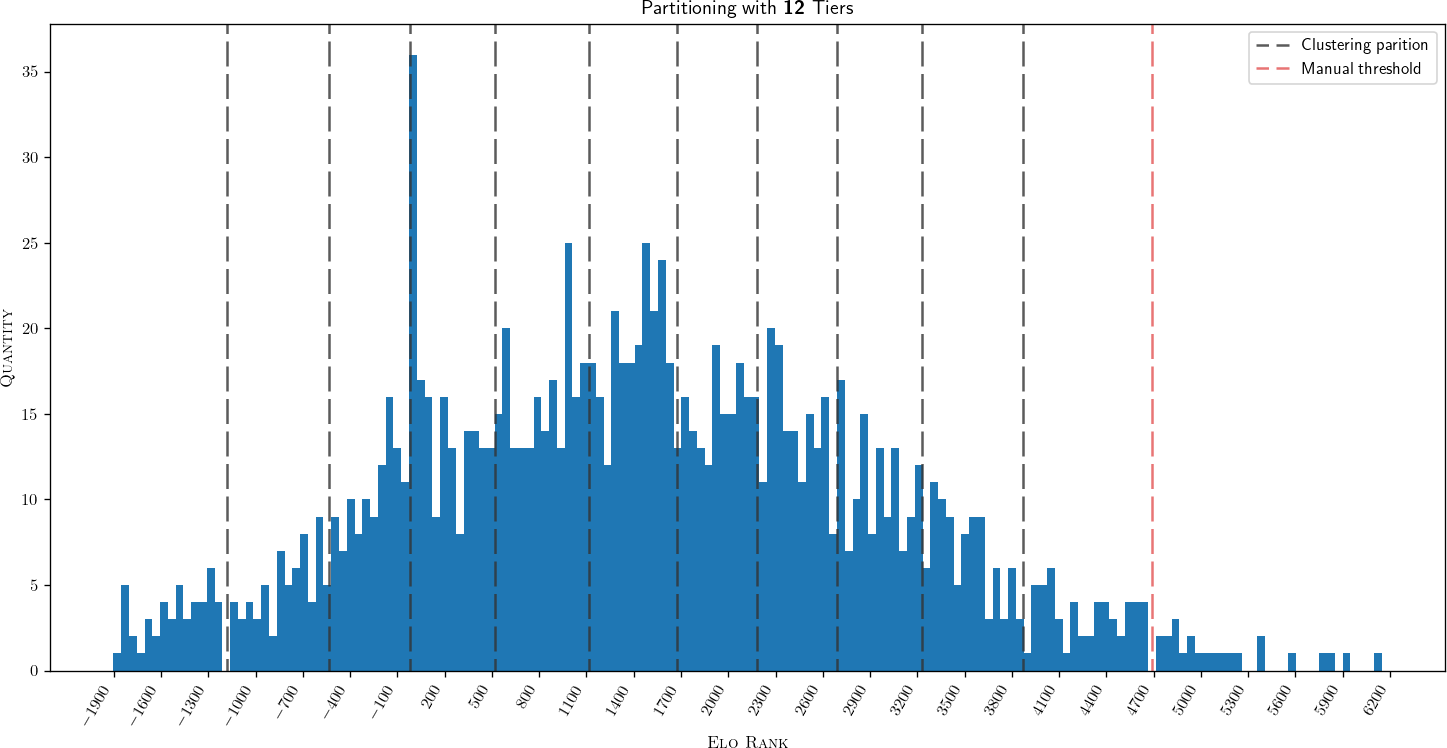
\includegraphics{Elo-Tier-Partition-12.png}}
	\caption{Class partitions (\Num{12}) for the \TERC candidate system}\label{fig:Partitions-TERC}
\end{figure}

\begin{figure}[htb]
	\centering
	\resizebox{\textwidth}{!}{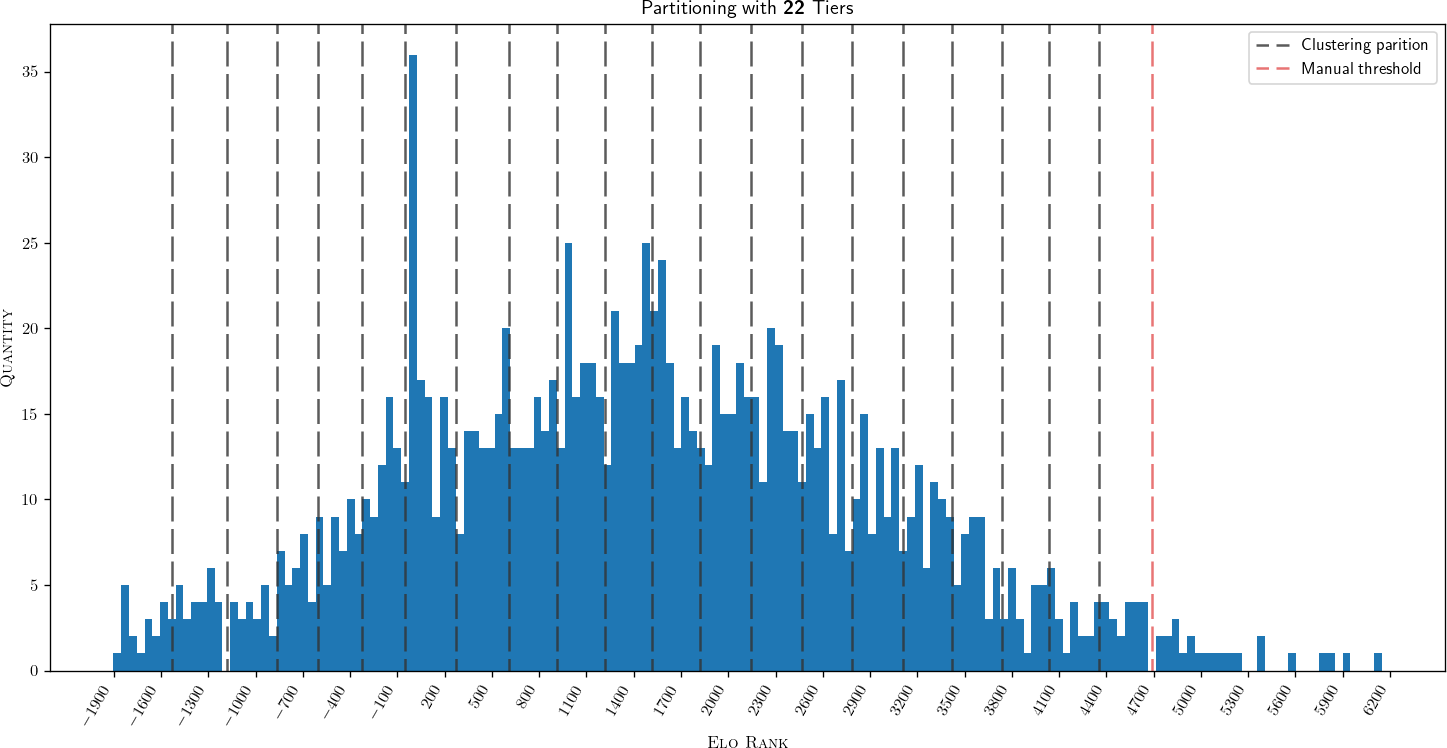
\includegraphics{Elo-Tier-Partition-22.png}}
	\caption{Class partitions (\Num{22}) for the \TER candidate system}\label{fig:Partitions-TER}
\end{figure}


\hypertarget{extraction-of-indicator-tags}{
\subsubsection{Additional Indicator Tags}\label{extraction-of-indicator-tags}}

The final feature extraction endeavor involves the columns, labeled
labeled \Column{Damage\ Tags}, \Column{Spellcasting\ Tags} and \Column{Trait\ Tags} indexed \IndexRange{66}{70}.
Each column contains a list of binary tags.
The existence of the tag in the list indicates a positive value for that binary indicator where as absence from the list indicates a negative value.
The column values represent an encoding of the ower set of possible binary indicators.
Hence, these columns can be expanded to extract an additional features as the form of multiple binary indicator columns.
All encoded binary indicators of these columns are extracted, totaling \Num{63} features combined.
This feature extraction nearly doubles the fully expanded dataset size, now totaling to \Num{136} features.
The fully extracted dataset is presented in Table \ref{tab:fully-extracted-dataset}.




\hypertarget{feature-selection}{%
\subsection{Feature Selection}\label{feature-selection}}

\begin{quote}
	{\itshape After extracting all possible features we perform feature selection.}
\end{quote}


\hypertarget{text-removal}{
\subsubsection{Elo elision}\label{elo-elision}}

First, the \Column{Elo Rank} column is dropped.
This is an obvious necessity, as inclusion of the values provides a linear mapping to the classes in \Column{Tier}.
Furthermore, a user of the classifier would not generally have access to the Elo rank.
Hence, the consideration of Elo rank values by an ML classifier would constitute an inappropriate feature.


\hypertarget{text-removal}{
\subsubsection{Text removal}\label{text-removal}}

Next the textual columns, \Column{Name} and \Column{Type} indexed \IndexRange{0}{1} are dropped from analysis.
These columns do not influence combat efficacy and are not convertible to a meaningful
numeric representation.
Their absence makes the machine learning process much smoother.


\hypertarget{uninformative-features}{
\subsubsection{Uninformative features}\label{uninformative-features}}

Subsequently,  all features extracted from the \Column{Damage Tag} and \Column{Spell Tag} columns are dropped.
These features had essentially no bearing on our first explored model (Multinomial Naive Bayes), and hence we decided to omit them from all future models for efficiency reasons.


\hypertarget{decorrelation}{
\subsubsection{Decorrelation}\label{decorrelation}}

For the final component of our feature selection process, we perform a "decorrelation" pass through the feature set.
If any pair of features have a correlation coefficient of \texttt{0.75} or higher, we drop one of the columns and use the other as a proxy.
Consequently, we dropped the features in Table \ref{tab:dropped-features}.


\hypertarget{final-datset-decription}{
\subsubsection{Final Dataset Description}\label{final-datset-decription}}

After feature extraction \emph{and} feature selection, the resulting dataset was comprised of \texttt{96} features.
See Table \ref{tab:final-dataset} for a reference of column names and types of the finalized dataset.
All the supervised learning models under considered outlined in Section \ref{model-specification} were trained on this dataset.


\section{Methods}


\hypertarget{datset-partitioning}{%
\subsection{Datset partitioning}\label{datset-partitioning}}

We take the prepared dataset and train multiple machine learning
classifiers. We use 80\% of the randomly permuted data as the training
set and the remaining 20\% as the test set. This partition data was
stratified by the \texttt{\textquotesingle{}Elo\ Rank\textquotesingle{}}
column to ensure that each tier is represented. Furthermore, we
partition the training set again, using 80\% as a learning set and the
remaining 20\% as the validation set. Model selection was performed on
the training set; comprised of the "learning" and validation subsets.

\begin{table}[!htbp] \centering 
\caption{Distribution for partitioning dataset,	stratified by \Column{Tier}.}
\label{tab:shrunk-observations}
\begin{longtable}[]{@{}lr@{}}
\toprule
Set & Ratio \\
\midrule
\endhead
Test & 20\% \\
Train & 80\% \\
Learn & 64\% \\
Validate & 16\% \\
\bottomrule
\end{longtable}
\end{table}

\hypertarget{model-specification}{%
\subsection{Model Specification}\label{model-specification}}
The following list contains the proposed machine learning models under consideration in our classifier search.
We will perform a hyperparameter search evaluate and then train each model under consideration.
Subsequently, the predictive capability of the models will be compared by their Precision, Recall, and F1 metrics.
The best performing classifier(s) will have their model(s) further tuned to produce a conclusive ``\DnD Monster Elo ranking classifier.''

\begin{enumerate}
	\def\labelenumi{\arabic{enumi}.}
	\item
	\textbf{Decision Tree:} Decision trees make extremely fast classifiers once constructed, but can be incredibly time consuming to build.
	We will try our luck with this model and see if an effective classifier could be built within a reasonable time frame.
	We might get a surprising result, but not placing a lot of hope in this model.
	\item
	\textbf{K Nearest Neighbors:} A very simple model with a theoretical bound on it's maximum inaccuracy.
	We will use this as our initial classifier to get our bearing and some quick benchmarking numbers.
	\item
	\textbf{Logistic Regression:} We recall from class that the a logistic regression
	can be an effective and efficient model for multi-class output, which
	our tier list is.
	This model will be considered because we suspected that the features have some linear, but not polynomial, relationship(s).
	The	logistic regression ought to capture and train well if linear relationships exists between the features and tier list labels.
	\item
	\textbf{Multinomial Naive Bayes:} Independent features are an important factor for the efficacy of Naive Bayes models.
	Naive Bayes models are supposed to train well on small number of observations.
	Our dataset will likely be just above the \texttt{1000} observation threshold, so we have high hopes that this model would train well.
	This will be our second model used to get quick benchmarking numbers.
	\item
	\textbf{Multi-layer Perceptron:} We wanted to experiment with the
	concept of artificial neural nets.
	The inclusion of this model will allow us to to get some experience with an instance of the buzzword-worthy model.
	Given the great flexibility of ANNs, we expected very good performance from this model.
	\item
	\textbf{Random Forest:} Given the unknown nature and limited domain knowledge that we could use to direct the machine learning process, the use of at least one ensemble learning technique seems to be a prudent choice.
	\item
	\textbf{Support Vector Machines:} In an ideal case, the data-set will be linearly separable in some hyperspace.
	If this ideal case matches the reality of the data-set, an SVM will perform exceptionally well, making it's inclusion is a natural choice.
\end{enumerate}

\hypertarget{model-selection}{%
\subsection{Model Selection}\label{model-selection}}

We performed model selection mainly by utilizing the \href{https://scikit-learn.org/stable/modules/generated/sklearn.model_selection.GridSearchCV.html}{\texttt{GridSearchCV}} function.
For each model, for both \TERC and \TER, a `wide and sparse sampling'' over the parameter space was performed.
Based on the results of this initial model selection, a subsequent ``denser'' hyperparameter search(es) were conducted, centered about the results from the initial sparse search.
This two pass approach proved quite effective both in terms of runtime efficiency and classifier efficacy.
The hyperparameters resulting from our model selection process can be found by referencing the executable file corresponding to the model listed in Table \ref{tab:hyperparameters}, and inspecting the definition of \texttt{hyperparameter\_values} within the file.


%Bibliography
\newpage
\medskip
\small
\bibliographystyle{IEEEtran}
\bibliography{references.bib}%
\clearpage


\section{Appendix}

\begin{table}[!htpb] \centering
\caption{%
\label{tab:matching}%
\bfseries Data source matching results.
}%
\begin{longtable}[]{@{}ccrrr@{}}
	\toprule
	\textbf{Source} & \textbf{Summary} & \textbf{Matched} & \textbf{Unmatched} & \textbf{Total} \\
	\midrule
	\FiveETools & Feature Set & 1630 &  703 & 2333 \\
	\hline \\[-3mm]
	\DnDCombat & Elo Rankings & 1630 & 1306 & 2936 \\
	\hline
\end{longtable}
\end{table}


\begin{table}[!htbp] \centering 
	\caption{\bfseries Initial Dataset} 
	\label{tab:initial-dataset}

\begin{footnotesize}
\begin{minipage}[b]{0.45\linewidth}\centering
\begin{longtable}[]{@{}rll@{}}
	\toprule
	\# & Column Label & Data Type \\
	\midrule
	\endhead
	0 & Name & Textual \\
	1 & Type & Textual \\
	2 & Size & Integral \\
	3 & Armor & Integral \\
	4 & Hit Points & Integral \\
	5 & Move Burrow & Integral \\
	6 & Move Climb & Integral \\
	7 & Move Fly & Integral \\
	8 & Move Swim & Integral \\
	9 & Move Walk & Integral \\
	10 & Stat Str & Integral \\
	11 & Stat Dex & Integral \\
	12 & Stat Con & Integral \\
	13 & Stat Int & Integral \\
	14 & Stat Wis & Integral \\
	15 & Stat Cha & Integral \\
	16 & Save Str & Integral \\
	17 & Save Dex & Integral \\
	18 & Save Con & Integral \\
	19 & Save Int & Integral \\
	20 & Save Wis & Integral \\
	21 & Save Cha & Integral \\
	22 & Blind Sight & Binary \\
	23 & Dark Vision & Binary \\
	24 & Tremorsense & Binary \\
	25 & True Sight & Binary \\
	26 & Immune Acid & Binary \\
	27 & Immune Bludgeoning & Binary \\
	28 & Immune Cold & Binary \\
	29 & Immune Fire & Binary \\
	30 & Immune Force & Binary \\
	31 & Immune Lightning & Binary \\
	32 & Immune Necrotic & Binary \\
	33 & Immune Piercing & Binary \\
	34 & Immune Poison & Binary \\
	35 & Immune Psychic & Binary \\
	\bottomrule
\end{longtable}
\end{minipage}
\hspace{0.5cm}
\begin{minipage}[b]{0.45\linewidth}\centering
\begin{longtable}{@{}rll@{}}
	\toprule
	\# & Column Label & Data Type \\
	\midrule
	\endhead
	36 & Immune Radiant & Binary \\
	37 & Immune Slashing & Binary \\
	38 & Immune Thunder & Binary \\
	39 & Resist Acid & Binary \\
	40 & Resist Bludgeoning & Binary \\
	41 & Resist Cold & Binary \\
	42 & Resist Fire & Binary \\
	43 & Resist Force & Binary \\
	44 & Resist Lightning & Binary \\
	45 & Resist Necrotic & Binary \\
	46 & Resist Piercing & Binary \\
	47 & Resist Poison & Binary \\
	48 & Resist Psychic & Binary \\
	49 & Resist Radiant & Binary \\
	50 & Resist Slashing & Binary \\
	51 & Resist Thunder & Binary \\
	52 & Cause Blinded & Binary \\
	53 & Cause Charmed & Binary \\
	54 & Cause Deafened & Binary \\
	55 & Cause Frightened & Binary \\
	56 & Cause Grappled & Binary \\
	57 & Cause Incapacitated & Binary \\
	58 & Cause Invisible & Binary \\
	59 & Cause Paralyzed & Binary \\
	60 & Cause Petrified & Binary \\
	61 & Cause Poisoned & Binary \\
	62 & Cause Prone & Binary \\
	63 & Cause Restrained & Binary \\
	64 & Cause Stunned & Binary \\
	65 & Cause Unconscious & Binary \\
	66 & Multiattack & Binary \\
	67 & Spellcasting & Binary \\
	68 & Damage Tags & Textual \\
	69 & Spellcasting Tags & Textual \\
	70 & Trait Tags & Textual \\
	71 & Elo Rank & Integral \\
	\bottomrule
\end{longtable}
\end{minipage}
\end{footnotesize}

\end{table}

\begin{table}[ht]
	\caption{\bfseries Fully Extracted Dataset}
	\label{tab:fully-extracted-dataset}
\begin{tiny}
\begin{minipage}[b]{0.45\linewidth}\centering
\begin{tabular}{@{}rll@{}}
	\toprule
	\# & Column Label & Data Type \\
	\midrule
	0 & Name & Textual \\
	1 & Type & Textual \\
	2 & Size & Integral \\
	3 & Armor & Integral \\
	4 & Hit Points & Integral \\
	5 & Move Burrow & Integral \\
	6 & Move Climb & Integral \\
	7 & Move Fly & Integral \\
	8 & Move Swim & Integral \\
	9 & Move Walk & Integral \\
	10 & Stat Str & Integral \\
	11 & Stat Dex & Integral \\
	12 & Stat Con & Integral \\
	13 & Stat Int & Integral \\
	14 & Stat Wis & Integral \\
	15 & Stat Cha & Integral \\
	16 & Save Str & Integral \\
	17 & Save Dex & Integral \\
	18 & Save Con & Integral \\
	19 & Save Int & Integral \\
	20 & Save Wis & Integral \\
	21 & Save Cha & Integral \\
	22 & Blind Sight & Binary \\
	23 & Dark Vision & Binary \\
	24 & Tremorsense & Binary \\
	25 & True Sight & Binary \\
	26 & Immune Acid & Binary \\
	27 & Immune Bludgeoning & Binary \\
	28 & Immune Cold & Binary \\
	29 & Immune Fire & Binary \\
	30 & Immune Force & Binary \\
	31 & Immune Lightning & Binary \\
	32 & Immune Necrotic & Binary \\
	33 & Immune Piercing & Binary \\
	34 & Immune Poison & Binary \\
	35 & Immune Psychic & Binary \\
	36 & Immune Radiant & Binary \\
	37 & Immune Slashing & Binary \\
	38 & Immune Thunder & Binary \\
	39 & Resist Acid & Binary \\
	40 & Resist Bludgeoning & Binary \\
	41 & Resist Cold & Binary \\
	42 & Resist Fire & Binary \\
	43 & Resist Force & Binary \\
	44 & Resist Lightning & Binary \\
	45 & Resist Necrotic & Binary \\
	46 & Resist Piercing & Binary \\
	47 & Resist Poison & Binary \\
	48 & Resist Psychic & Binary \\
	49 & Resist Radiant & Binary \\
	50 & Resist Slashing & Binary \\
	51 & Resist Thunder & Binary \\
	52 & Cause Blinded & Binary \\
	53 & Cause Charmed & Binary \\
	54 & Cause Deafened & Binary \\
	55 & Cause Frightened & Binary \\
	56 & Cause Grappled & Binary \\
	57 & Cause Incapacitated & Binary \\
	58 & Cause Invisible & Binary \\
	59 & Cause Paralyzed & Binary \\
	60 & Cause Petrified & Binary \\
	61 & Cause Poisoned & Binary \\
	62 & Cause Prone & Binary \\
	63 & Cause Restrained & Binary \\
	64 & Cause Stunned & Binary \\
	65 & Cause Unconscious & Binary \\
	66 & Multiattack & Binary \\
	67 & Spellcasting & Binary \\
	\bottomrule
\end{tabular}
\end{minipage}
\hspace{0.5cm}
\begin{minipage}[b]{0.45\linewidth}\centering
\begin{tabular}{@{}rll@{}}
	\toprule
	\# & Column Label & Data Type \\
	\midrule
	68 & Damage\_A & Binary \\
	69 & Damage\_B & Binary \\
	70 & Damage\_C & Binary \\
	71 & Damage\_F & Binary \\
	72 & Damage\_I & Binary \\
	73 & Damage\_L & Binary \\
	74 & Damage\_N & Binary \\
	75 & Damage\_O & Binary \\
	76 & Damage\_P & Binary \\
	77 & Damage\_R & Binary \\
	78 & Damage\_S & Binary \\
	79 & Damage\_T & Binary \\
	80 & Damage\_Y & Binary \\
	81 & Spellcasting\_CA & Binary \\
	82 & Spellcasting\_CB & Binary \\
	83 & Spellcasting\_CC & Binary \\
	84 & Spellcasting\_CD & Binary \\
	85 & Spellcasting\_CL & Binary \\
	86 & Spellcasting\_CP & Binary \\
	87 & Spellcasting\_CR & Binary \\
	88 & Spellcasting\_CS & Binary \\
	89 & Spellcasting\_CW & Binary \\
	90 & Spellcasting\_F & Binary \\
	91 & Spellcasting\_I & Binary \\
	92 & Spellcasting\_P & Binary \\
	93 & Spellcasting\_S & Binary \\
	94 & Aggressive & Binary \\
	95 & Ambusher & Binary \\
	96 & Amorphous & Binary \\
	97 & Amphibious & Binary \\
	98 & Antimagic Susceptibility & Binary \\
	99 & Brute & Binary \\
	100 & Charge & Binary \\
	101 & Damage Absorption & Binary \\
	102 & Death Burst & Binary \\
	103 & Devil's Sight & Binary \\
	104 & False Appearance & Binary \\
	105 & Fey Ancestry & Binary \\
	106 & Flyby & Binary \\
	107 & Hold Breath & Binary \\
	108 & Illumination & Binary \\
	109 & Immutable Form & Binary \\
	110 & Incorporeal Movement & Binary \\
	111 & Keen Senses & Binary \\
	112 & Legendary Resistances & Binary \\
	113 & Light Sensitivity & Binary \\
	114 & Magic Resistance & Binary \\
	115 & Magic Weapons & Binary \\
	116 & Pack Tactics & Binary \\
	117 & Pounce & Binary \\
	118 & Rampage & Binary \\
	119 & Reckless & Binary \\
	120 & Regeneration & Binary \\
	121 & Rejuvenation & Binary \\
	122 & Shapechanger & Binary \\
	123 & Siege Monster & Binary \\
	124 & Sneak Attack & Binary \\
	125 & Spell Immunity & Binary \\
	126 & Spider Climb & Binary \\
	127 & Sunlight Sensitivity & Binary \\
	128 & Turn Immunity & Binary \\
	129 & Turn Resistance & Binary \\
	130 & Undead Fortitude & Binary \\
	131 & Water Breathing & Binary \\
	132 & Web Sense & Binary \\
	133 & Web Walker & Binary \\
	134 & Elo Rank & Integral \\
	135 & Tier & Integral \\
	\bottomrule
\end{tabular}
\end{minipage}
\end{tiny}

\end{table}

\begin{table}[!htbp] \centering 
	\caption{Dropped highly correlated features and their proxy}
	\label{tab:dropped-features}
	
\begin{longtable}[]{@{}ll@{}}
	\toprule
	Proxy & Dropped Feature \\
	\midrule
	\endhead
	Hit Points & Size \\
	Hit Points & Stat Str \\
	Hit Points & Stat Con \\
	Stat Cha & Stat Int \\
	Resist Fire & Resist Cold \\
	Resist Fire & Resist Lightning \\
	Resist Acid & Resist Thunder \\
	Resist Acid & Incorporeal Movement \\
	Damage Absorption & Immutable Form \\
	Spell Immunity & Immune Force \\
	Web Sense & Web Walker \\
	\bottomrule
\end{longtable}

\end{table}


\begin{table}[!htbp] \centering 
	\caption{\bfseries Final Dataset}
	\label{tab:final-dataset}
\begin{scriptsize}
\begin{minipage}[b]{0.45\linewidth}\centering
\begin{longtable}[]{@{}rll@{}}
	\toprule
	\# & Column Label & Data Type \\
	\midrule
	\endhead
	0 & Armor & Integral \\
	1 & Hit Points & Integral \\
	2 & Move Burrow & Integral \\
	3 & Move Climb & Integral \\
	4 & Move Fly & Integral \\
	5 & Move Swim & Integral \\
	6 & Move Walk & Integral \\
	7 & Stat Dex & Integral \\
	8 & Stat Wis & Integral \\
	9 & Stat Cha & Integral \\
	10 & Save Str & Integral \\
	11 & Save Dex & Integral \\
	12 & Save Con & Integral \\
	13 & Save Int & Integral \\
	14 & Save Wis & Integral \\
	15 & Save Cha & Integral \\
	16 & Blind Sight & Binary \\
	17 & Dark Vision & Binary \\
	18 & Tremorsense & Binary \\
	19 & True Sight & Binary \\
	20 & Immune Acid & Binary \\
	21 & Immune Bludgeoning & Binary \\
	22 & Immune Cold & Binary \\
	23 & Immune Fire & Binary \\
	24 & Immune Lightning & Binary \\
	25 & Immune Necrotic & Binary \\
	26 & Immune Piercing & Binary \\
	27 & Immune Poison & Binary \\
	28 & Immune Psychic & Binary \\
	29 & Immune Radiant & Binary \\
	30 & Immune Slashing & Binary \\
	31 & Immune Thunder & Binary \\
	32 & Resist Bludgeoning & Binary \\
	33 & Resist Cold & Binary \\
	34 & Resist Force & Binary \\
	35 & Resist Necrotic & Binary \\
	36 & Resist Piercing & Binary \\
	37 & Resist Poison & Binary \\
	38 & Resist Psychic & Binary \\
	39 & Resist Radiant & Binary \\
	40 & Resist Slashing & Binary \\
	41 & Cause Blinded & Binary \\
	42 & Cause Charmed & Binary \\
	43 & Cause Deafened & Binary \\
	44 & Cause Frightened & Binary \\
	45 & Cause Grappled & Binary \\
	46 & Cause Incapacitated & Binary \\
	47 & Cause Invisible & Binary \\
	\bottomrule
\end{longtable}
\end{minipage}
\hspace{0.5cm}
\begin{minipage}[b]{0.45\linewidth}\centering
\begin{longtable}{@{}rll@{}}
	\toprule
	\# & Column Label & Data Type \\
	\midrule
	\endhead
	48 & Cause Paralyzed & Binary \\
	49 & Cause Petrified & Binary \\
	50 & Cause Poisoned & Binary \\
	51 & Cause Prone & Binary \\
	52 & Cause Restrained & Binary \\
	53 & Cause Stunned & Binary \\
	54 & Cause Unconscious & Binary \\
	55 & Multiattack & Binary \\
	56 & Spellcasting & Binary \\
	57 & Aggressive & Binary \\
	58 & Ambusher & Binary \\
	59 & Amorphous & Binary \\
	60 & Amphibious & Binary \\
	61 & Antimagic Susceptibility & Binary \\
	62 & Brute & Binary \\
	63 & Charge & Binary \\
	64 & Death Burst & Binary \\
	65 & Devil's Sight & Binary \\
	66 & False Appearance & Binary \\
	67 & Fey Ancestry & Binary \\
	68 & Flyby & Binary \\
	69 & Hold Breath & Binary \\
	70 & Illumination & Binary \\
	71 & Immutable Form & Binary \\
	72 & Incorporeal Movement & Binary \\
	73 & Keen Senses & Binary \\
	74 & Legendary Resistances & Binary \\
	75 & Light Sensitivity & Binary \\
	76 & Magic Resistance & Binary \\
	77 & Magic Weapons & Binary \\
	78 & Pack Tactics & Binary \\
	79 & Pounce & Binary \\
	80 & Rampage & Binary \\
	81 & Reckless & Binary \\
	82 & Regeneration & Binary \\
	83 & Rejuvenation & Binary \\
	84 & Shapechanger & Binary \\
	85 & Siege Monster & Binary \\
	86 & Sneak Attack & Binary \\
	87 & Spell Immunity & Binary \\
	88 & Spider Climb & Binary \\
	89 & Sunlight Sensitivity & Binary \\
	90 & Turn Immunity & Binary \\
	91 & Turn Resistance & Binary \\
	92 & Undead Fortitude & Binary \\
	93 & Water Breathing & Binary \\
	94 & Web Walker & Binary \\
	95 & Tier & Integral \\
	\bottomrule
\end{longtable}
\end{minipage}
\end{scriptsize}

\end{table}


\begin{table}[!htbp] \centering 
	\caption{ Model \& file containing corresponding \texttt{hyperparameter\_values} definition.}
	\label{tab:hyperparameters}
\begin{longtable}[]{@{}ll@{}}
\toprule
Model Name & Executable File \\
\midrule
\endhead
Decision Tree           & \href{https://github.com/recursion-ninja/CSc-CSc-74020/tree/master/src/classification/model_DecisionTree.py       }{\texttt{classification/model\_DecisionTree.py}} \\
K Nearest Neighbors     & \href{https://github.com/recursion-ninja/CSc-CSc-74020/tree/master/src/classification/model_KNN.py                }{\texttt{classification/model\_KNN.py}} \\
Logistic Regression     & \href{https://github.com/recursion-ninja/CSc-CSc-74020/tree/master/src/classification/model_LogisticRegression.py }{\texttt{classification/model\_LogisticRegression.py}} \\
Multinomial Naive Bayes & \href{https://github.com/recursion-ninja/CSc-CSc-74020/tree/master/src/classification/model_NaiveBayes.py         }{\texttt{classification/model\_NaiveBayes.py}} \\
Multi-layer Perceptron  & \href{https://github.com/recursion-ninja/CSc-CSc-74020/tree/master/src/classification/model_NeuralNetwork.py      }{\texttt{classification/model\_NeuralNetwork.py}} \\
Random Forest           & \href{https://github.com/recursion-ninja/CSc-CSc-74020/tree/master/src/classification/model_RandomForest.py       }{\texttt{classification/model\_RandomForest.py}} \\
Support Vector Machines & \href{https://github.com/recursion-ninja/CSc-CSc-74020/tree/master/src/classification/model_SVM.py                }{\texttt{classification/model\_SVM.py}} \\
\bottomrule
\end{longtable}
\end{table}

\end{document}
